%************************************************
\chapter{Literature Review}\label{ch:litreview}
%************************************************
This literature review will first summarise the current state of the art in data integration within the rail domain, before moving on to discuss the costs and benefits of greater integration. Linked data and ontology will be introduced as a means of achieving improved integration between data resources, and cases studies from other industries, which have adopted ontology for integration will be examined and conclusions drawn. The discussion will conclude with a summary of how the lessons learnt may be applied to GB rail.
% Lastly a number of techniques used throughout this thesis will be explained.

In the last twenty years the world outside of the rail industry has changed significantly, with information communication technology becoming all pervasive, however the rail industry has been slower to adapt. Although customer information is now commonly provided electronically and commodity software platforms provide multimodal journey planning, these services are only as good as the data fed to them. Within the industry however ICT systems remain siloed, with advances made in the gathering of data but exploitation being limited by system boundaries and commercial barriers. 

\section{State of the Industry}
\label{state}

The Mc Nulty report, a study into value for money offered by GBRail, \citep{DepartmentforTransport2011}, found that:
\begin{quote}
    The effectiveness of the industry’s IS is inhibited by a suite of legacy systems that are expensive to run, unable to communicate with new technology and encourage users to develop a wide range of bespoke local systems to overcome limitations. Many legacy systems were created and managed in company silos, with only a few systems crossing industry boundaries.
\end{quote}

The report goes on to conclude: 
\begin{quote}
Information systems are at the heart of a more efficient railway that delivers value for money. Allowing the railway’s existing IS to continue unreconstructed will increase cost, reduce efficiency and undermine customer service. In contrast, the replacement of legacy systems and the exploitation of new technology will generate improved value for money.
\end{quote}
Also proposed in the report was the creation of the Rail Delivery Group, an industry body representing infrastructure, freight, and passenger operators\footnote{Further information may be found at: \url{http://orr.gov.uk/about-orr/who-we-work-with/industry-organisations/rail-delivery-group}}. Another report, created as a response to the The Rail Technical Strategy \citep{TechnicalStrategyLeadershipGroup2012b}, identifies a need for better data integration, stating that:

\begin{quote}
Over 130 information systems maintained by approximately 20 suppliers were in operation in 2011. Maintaining individual legacy systems is expensive and inefficient. Information cannot be shared or exploited efficiently and this inhibits whole-system approaches for technology-based improvements. 
\end{quote}

The \citet{RDG2017} proposes in the \say{Capability Delivery Plan} that: \say{Standards will allow information to be interpreted and combined more easily delivering new insights and intelligence to the industry.}. At the present time this goal is still outstanding. 

The issue of lock in to proprietary systems and the creation of data silos is examined in \citet{Joh13}, which states that
\begin{quote}
    Where electronic data exchange standards for rail do exist, many are proprietary binary formats used to provide point-to-point interfaces between specific systems and not intended for use in a generalised context.
\end{quote}
\citet{Verstichel2011a} finds a need for improved data integration in the larger European rail domain: ``Industry-wide integration in the information domain is only in its infancy. From an efficiency point of view, this field leaves much room for improvement (as did the integration in the mechanical and electrical domain). ''

 \citet{Morris2014} discusses the rising rail ridership in the UK, along with the need for improved efficiency. This trend continues as shown by the official statistics from the Office of Road and Rail, \citet{OfficeofRoad&Rail2016}, with 1.7 billion journeys having been made in the financial year 2016-17, up 0.8\% from the previous financial year; this marks the highest ever number of journeys on the UK rail network, since statistics started being collected in 1950. However it should be noted that this is also the smallest year on year increase since 2009-10.

Since the benefits of improved data integration have been identified, Network Rail the UK infrastructure operator, has taken steps to improve data integration using conventional means. A good example of this is the Linear Asset Decision Support solution, internally referred to as LADS\footnote{technically, LADS is an implementation by Capgemini of Bently Optram}, which brings together fourteen asset information systems, including the Rail Defect Management System, as part of the Offering Rail Better Information Services (ORBIS) program. This system has two front-ends; a hand-held system which can be used on ruggedized tablets track side to access information about nearby assets, and a desktop version for planning purposes. The system can show amongst other things:
\begin{itemize}
    \item Video (or stills) of the track, taken from New Measurement Train;
    \item Track Geometry measurements, also from the New Measurement Train;
    \item Track defect data and reports;
    \item Asset Locations;
    \item Asset type and age;
    \item Maintenance history.  
\end{itemize} 
These datasets are shown together in a ``swim lane'' view. This proprietary system covers the asset maintenance domain and will need extensive development to add new data sources or outputs. 
 
The amount of data used within the rail domain has increased rapidly with time. As it has become possible to collect more data on asset condition the volumes of data relating to each asset have grown, for example the work done in response to the \say{FuTRO Universal Data Challenge} reported by \citet{Tutcher2015a} suggests that large volumes of data\footnote{up to\say{15 seconds of data, sampled at 4kHz, for eight sensors}, though this can be down-sampled.} would need to be recorded every time a sets of points, also refereed to as switches or turnouts, moved anywhere on the rail network. Techniques such as alternating current field measurement sensor (ACFM) as discussed by \citet{Rowshandel2013} also produce large volumes of data, in this case relating to rail condition. Others sources of high volumes of data include ground penetrating radar, to assess trackbed condition, as reported by \citet{eriksen2004improved}. An assessment of the growing volume of data in the rail domain in an American context was performed by \citet{Zarembski}, which finds condition monitoring to be a likely source of growth. The European rail network is considered in \citet{Nunez2014}, which also studies data used for maintenance in the rail domain, taking as a case study the Dutch Rail Network. In the UK large volumes of  data are collected by the New Measurement Train and significant value could be added to this if it were easier to match readings with the assets to which they pertained.

The current work flow with regards wheel impact load detection is an example of less successful integration, which was described by \citet{Tutcher2015} as  ``several interfaces between machine and human operator railway data management exist as wheel impact data is taken from its silo, manually compared to train running information in another silo, and finally input into a maintenance system silo''. Wheel impact load is important because it detects when train wheels are damaged, thus in turn causing damage to the track and train alongside causing discomfort to passengers.

\subsection{Information Security}

Alongside the growth in data stored electronically comes a second, related, issue; that of IT security. As data has become more distributed and greater use is made of the public internet further precautions are required. The importance of this in the rail domain is discussed by \citet{Depar2016}, and further discussions in the context of the cybersecurity of signalling systems may be found in \citep{BloomField2016} and \citep{Chen2015}. In \citet{Chen2015} the security of passenger information systems is also considered.

\section{Ontology}\label{onto}
In \autoref{ch:intro} of this document ontology was defined as: 
\begin{quote}
\emph{an explicit specification of a conceptualization}
\end{quote}
The author of that quote, Tom Gruber, has gone on to provide a more complete definition in \citep{Gru09}. 

\begin{quote}
\begin{itemize}
\item An ontology defines (specifies) the concepts, relationships, and other distinctions that are relevant for modelling a domain.
\item The specification takes the form of the definitions of representational vocabulary (classes, relations, and so forth), which provide meanings for the vocabulary and formal constraints on its coherent use
\end{itemize}
\end{quote}

Data integration was one of the first benefits of ontology to be identified, as early as 1991 and was already under discussion \citep{Siegel1991}, along with several other uses cases that remain relevant today. \citet{Siegel1991} aimed to enable the \say{integration of multiple disparate database systems} by using a ``common metadata vocabulary'' and suggested that \say{global ontology to provide the common vocabulary and all component systems must provide semantic mappings to that global ontology}. This approach remains broadly valid today, though the available implementation toolsets have improved significantly. 

An ontology could be described a means of storing a view of the world, in this context, it stores information, not simply data. Beyond that ontologies allow reasoning to be performed and new information to be inferred from the facts and rules it contains. This can be used simply to categorise objects, itself a powerful mechanism e.g. things may be classified as faulty or working, according to their properties. Rules can however be used to abstract other logic; would it be wise to offer insurance based on the provided circumstances for example. Reasoning allows strict mathematical logic to produce results, for example: \(\forall L \exists D \cap T \) where L is life, D is Death and T is taxes represents the proverb: \say{In this world nothing can be said to be certain, except death and taxes}. The development of ontologies from First Order Logic is covered in depth in by \citet{baader_calvanese_mcguinness_nardi_patel-schneider_2007}.

\subsection{Ontology Reasoning}
In the context of computational ontology, reasoning is used to imply facts not originally known or stored based on existing facts in the triple store. For example, if you know that every human has exactly one biological mother who is female and one father who is male, persons F and M are C's parents, and that person M is male, you may infer that person F is female.  This is discussed in depth in section 2.4.5 of \citet{Tutcher2015}. Reasoning can also be used to ascertain whether the concepts from two different models represent the same thing, or for classification of objects against a hierarchy within the ontology model. Reasoning has been used for purposes as diverse as ascertaining the correct pension to pay someone, based on their employment history, through to assigning biological systems to groups. In the rail context it has been used in multiple projects to ascertain if a combination of circumstances implies a fault.

\subsection{Ontology related terminology}

When discussing ontology the thesis will use the following terminology:

\subsubsection{Triples}\label{sec:trip}
When ontologies are stored electronically they take the form of triples, a statement broken into three parts, the subject, the predicate and the object as illustrated in \autoref{fig:joffrey}. Anything refereed to by a triple should have a unique identifier, known in this context as a Uniform Resource Identifier or URI. The W3C recommends that these URI's take the form of Uniform Resource Locators commonly abbreviated URL and that further more these Uniform Resource Locators point to a resolvable domain name. Whilst this is considered best practice it is entirely possible to create an ontology were the URIs are not URLs. Each part of a triple can be a URI itself, however, it is also possible for the object of a triple to be a simple value or a ``blank node'', that is a node with no name, used to link to further nodes.
\begin{figure}[hb]
    \myfloatalign
    {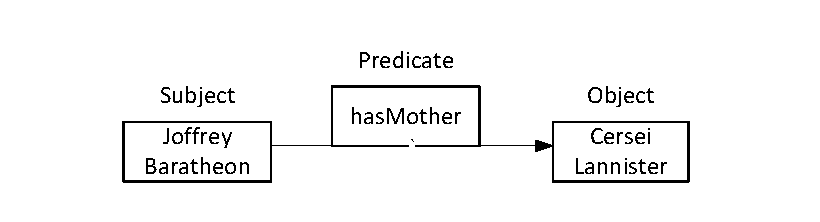
\includegraphics[width=\linewidth,keepaspectratio]{gfx/JofferyTriple}} 
    \caption[Triple]{The parts of a triple. Note that the content of each box is commonly a URI}
    \label{fig:joffrey}
\end{figure}
In this context a triple can also be thought of as a directed graph, in which the Subject and Object are both nodes.

\subsubsection{Tbox and ABox}
Throughout this discussion the terms ``TBox'' and ``ABox'' will be used. The TBox or ``Terminology'' box refers to that part of the ontology that holds the definitions and concepts. The statement ``Humans are a type of animal'' would generally belong in the TBox of an ontology. The ABox or assertion box holds assertions made using that knowledge, one such assertion could be \say{Chris Morris is a human}. In a relational database terms TBoxes and ABoxes are comparable to the schema (TBox) and the data (ABox).

\subsubsection{Expressivity}
Ontology expressivity is the complexity of the concepts that can be represented in a given form. Expressivity is generally described using Description Logic (refereed to in the literature as a DL), which are in turn decidable fragments of First-Order Logic. Different DLs represent different sub-sets of First-Order Logic and are annotated according to how expensive they are. 
\citet{Horridge2012} discusses some common levels of expressivity, in section 2 of the paper:
\begin{itemize}
    \item  \(\mathcal{AL}\) Is amongst the most limited, supporting:
        \begin{itemize}
            \item   Intersection  \(\cap\);
            \item   Universal quantification (All Value From) \( \forall \);
            \item   Limited existential quantification, with restrictions \( \exists\) ;
            \item   Atomic Negation \(\neg \) .
        \end{itemize}        
        The limitations of \(\mathcal{AL}\) description logic restrict the complexity of the concepts that can be encoded and, as such this DL is not commonly used, aside from as a basis for more complete description logics.
        \item With Full Negation this becomes  \(\mathcal{ALC}\). This means that any concept, not just atomic concepts (generally variables in first order logic), can be negated. Certain approaches, such as that discussed by \citet{Meyer2006} limit themselves to the \(\mathcal{ALC}\) description logic, since most operations can be performed on it in polynomial time.
        \item Adding hierarchy - sub-properties makes this \(\mathcal{ALCH}\)
        \item Adding nominals (only one can exist), inverse properties (lifts is the inverse of liftedBy for example) and numerical restrictions gives - \(\mathcal{ALCHOIN}\). 
        \item Add transitive properties, for example \say{if x is a part of y and y is a part z then x is a part of z} gives \(\mathcal{SHOIN}\), because \(\mathcal{ALC}\) with transitive properties is abbreviated \(\mathcal{S}\). As discussed by \citet{Horrocks2006a} \(\mathcal{SHOIN}\) underpins OWL 1 and thus is very widely used.  
\end{itemize}
More expressive DLs exist, but increasing the complexity of the concepts expressed also increases the complexity (and thus computational time required) of reasoning. A more expressive DL still, \(\mathcal{SROIQ}\), is used as the basis of the OWL 2 (discussed in \autoref{sec:standards}). This DL allows for properties to be, disjoint, reflexive, irreflexive or antisymmetric as well as all the properties found in \(\mathcal{SHOIN}\). For a description of \(\mathcal{SROIQ}\) see \citet{Horridge2012} section 2 or for greater depth: \citet{Horrocks2006}. A tool for the comparison of various description logics may be found at: \url{http://www.cs.man.ac.uk/~ezolin/dl/}.

Choice of level of expressivity is very important in ontology design and is considered in depth by \citet{Tutcher2015}. In that work the danger of allowing too much expressivity and making it either difficult or impossible to use automated tools to carry out reasoning is discussed. Since it is expected that reasoning will be used over ontologies in the rail domain, the question of expressivity will be further considered in the remainder of this thesis.

\subsubsection{Upper Ontologies}
When technology first made it possible to store logic and ontologies electronically and to perform reasoning computationally many studies proposed upper ontologies. That is ontologies that, in keeping with the philosophical basis of the term, aimed to be \say{Theories of everything}, to hold all of humanities knowledge. This resulted in several projects; foremost amongst the early studies was SUMO, the suggested upper merged ontology, proposed by \cite{Niles2001}. Latterly a number of other upper ontologies have emerged, such as  BFO or basic formal ontology, which is considered in the context of the biomedical domain by \citet{Grenon2004}. The advantage of using a common upper ontology is improved integration \emph{between different ontologies}. It can be seen that whilst this idea is much discussed in the literature examples of its' practical implementation are harder to find.

\section{Standards for data integration}\label{sec:standards}
One domain in which significant progress has been made is that of standards for interoperability of ontologies and the formats in which they are stored.

\subsection{Basic Standards}
There are several low level standards upon which the other standards this document will consider are built.

\subsubsection{XML}
Several current standards in use within the industry are based upon Extensible Mark-up Language (XML). XML is defined by \citet{W3.org2013} as \say{application profile or restricted form of SGML, the Standard Generalized Markup Language [ISO 8879]}. Standard Generalized Markup Language (SGML) is in turn a means of specifying a document structure, of which HTML (Hyper Text Markup Language) is the best known. XML is a data description language which uses SGML, effectively it is a way of specifying a data transfer. It is comparatively verbose and can, though does not have to be designed such that it is human readable.  

\subsubsection{Resource Description Framework}
The Resource Description Framework, here on referred to as RDF, is a standard that can be used for the interchange of linked data and ontologies. Defined by the W3C a guide is available in \citet{Wood14}. RDF was initially used primarily for the provision of metadata from conventional websites and is still commonly used within the semantic web. RDF forms the basis for other standards, most notably Web Ontology Language \autoref{sec:OWL}. It should be noted that while it is quite possible to use RDF triples out of an ontology driven environment, RDF alone does not provide sufficient contextual information to enable reasoning operations to take place.

\subsubsection{Web Ontology Language}\label{sec:OWL}
OWL or Web Ontology Language has become the standard for ontologies which are to be shared online. OWL is a recommendation from the W3C, the de facto standards body for web standards. Other domain specific languages have been developed in the past, sometimes with greater expressivity than OWL, however these have not seen wide adoption. The OWL 2 was released in 2012.

The OWL guidance document by \citet{McGuinness04} explores the comparison between XML and OWL, specifically it poses the question \say{What does this buy me that XML and XML Schema don\'t?} and suggests firstly that OWL (and this point applies equally to ontologies in general) provides a form of knowledge representation, not just a schema. From a schema you know how to respond to an expected message, but nothing else is possible. Secondly the same document also states that once a reasoner has been constructed it can be applied to many domain ontologies, thus promoting reuse.

The specification for OWL 2 may be found in \cite{Parsia:09:OWO} and a guide in \citet{Parsia12}. OWL 2 became available during the development of the RaCoOn ontologies and has the following ``Profiles'' available, the details of which are considered by \citet{Parsia12}:

\begin{itemize}
    \item OWL 2 Full Consistency checking and entailment checking are un-decidable at this level, however this offers the maximum possible expressivity of any profile. 
    \item OWL 2 EL This uses a DL called \(\mathcal{EL}^{++}\) - discussed in \citet{Baader2005} \(\mathcal{EL}^{++}\) is a good compromise of tractability and expressivity in particular because it can be reasoned over in polynomial time, whilst still capturing the complexity of large ontologies. This profile was designed with the biomedical domain in mind, where it is used extensively, since ontologies in this domain often have complex T-Boxes and very large A-Boxes;
    \item OWL 2 QL As stated in \citep{Parsia12} this DL \say{can be realized using standard relational database technology}. The intended use case of this profile is to build on the years of development and optimisation around classic relational databases, by implementing Ontologies that leverage these systems as their datastores;
    \item OWL 2 RL is more restrictive than the previous two profiles, aimed at working with RDF data at scale, giving fast reasoning over large datasets;
    \item OWL DL ``Direct Semantics'' is the subset of OWL 2 which is required to implement \(\mathcal{SROIQ}\). This is larger than any of the other profiles listed above, but is still only a subset of OWL 2 Full. Ontologies complying with the DL sub-language of OWL (as opposed to OWL 2) are automatically valid OWL 2 DL ontologies, which is useful for backward compatibility. 
\end{itemize}

\subsubsection{SPARQL}
\label{sec:lit_rv_sparql}
SPARQL, a recursive acronym meaning ``SPARQL Protocol and RDF Query Language'', is a language used to query ontology data-stores. It can perform  \say{Create, Read, Update and Delete} or CRUD operations, an overview is provided by the \citet{5403219}. Syntactically and functionally SPARQL bears comparison to SQL, the Structured Query Language used with relational databases. Both facilitate CRUD operations including very complex criteria for selection, however SPARQL differs in that the data to be queried will always be RDF triples. 

\subsubsection{GEO SPARQL}
Geo-SPARQL is an extension of SPARQL, as discussed in \autoref{sec:lit_rv_sparql} for handling geographic data. It is defined by the Open Geospatial Consortium\footnote{The definition is available from \url{http://www.opengis.net/doc/IS/geosparql/1.0}} in \citet{Perry2012}. This makes it possible to ascertain if a given point is within an area, if two areas intersect or to find the distance between two points, for example. It can use a number of different coordinate systems and convert between them. It is used, in conjunction with SPARQL, to write more complex queries which can take into account an item's location.

\section{Software tools}
The commercial market for ontology related software has grown significantly in recent years and there is now a selection of tools available for many different ontology operations. Ontology editing tools, reasoners and triple stores are all competitive market places, with both commercial and open source products available in all spheres. Another area in which a range of tools is available is that of moving from relational database to ontology and linked data. If the database schema is taken as the T-Box and the row data the A-Box, then it is possible to design an automated tool to do exactly this and make the data available as an ontology. A method for recording the mappings of relational databases to ontologies is discussed by \citet{Dimou2014}, and a survey of the available tools for automating the process is available in: \citep{Spanos2012}. As discussed throughout the literature, a fully automated approach often produces a slightly idiosyncratic T-Box and better results may be achieved by running a first automated pass then a human intervention to improve the model.

Many software tools were required for project. Some such as the integrated development environment, were selected purely on the grounds of experience; familiarity with a tool is very valuable on its own, thus visual studio\footnote{details of this product and the various editions available are available from \url{https://www.visualstudio.com/}} and C\# were used for the majority of the software development. Another tool required was an ontology editor, for making additions and alterations to the rail core ontologies. Many such tools exist and \citet{Erlingsson2016} provides a review of the most popular. Top Braid composer Maestro Edition \footnote{Available from \url{https://www.topquadrant.com/tools/modeling-topbraid-composer-standard-edition/}} was selected for this project owing to the comparative speed with which it was possible to add large numbers of individuals alongside the useful visualisation functionality. 

In order as to store data in a linked format it is necessary to use a triple store. A triple store is a data store which holds information as triples, as discussed in \autoref{sec:trip}. All common triple stores provide basic CRUD functionality, however they can be differentiated on a number of grounds: 

\begin{itemize}    
    \item Cost and License. Some are open source, others offer free trials or reduced academic licenses. Others are commercial products, commonly having significant licensing costs;
    \item Performance. How rapidly operations can be performed on given hardware. This includes not just CRUD operations but also reasoning over the ontology;
    \item Security. Many triple stores offer some form of access control, with varying levels of granularity. Some triple stores support access control per graph, some allow for multiple datastores to be hosted by the same server with different permissions and access control lists. Triple stores can also have groups and roles, similar to traditional relational databases, to allow bulk management of user access;
    \item Extent of available support. Triple stores range from abandoned academic projects to commercial offerings with support contracts;
    \item Compatibility. This consideration is key when the other technologies in the system have already been selected.
    \item Extra features. Many triple stores offer features beyond CRUD, not all of which are relevant to all implementations;
\end{itemize}

The market for triple stores is evolving rapidity at present and a number of new products are emerging, however, due to the existence of previous work on which this thesis was based, Stardog\footnote{Made by Clarke \& Persia, download and further details available from: \url{http://www.stardog.com/}} was selected. This was then assessed on the criteria above:

\begin{description}    
    \item[Cost and License] A \say{community edition} is available for free. Certain projects required features not available in that edition, however and for that an arrangement was made with Clarke \& Persia.
    \item[Performance] No benchmarking was undertaken by this project;
    \item[Security] Stardog offers per graph security. Each database can contain many graphs, if the user desires.
    \item[Support] Extensive documentation is provided, additionally questions are always quickly responded to in the public support group.
    \item[Compatibility] Interfaces exist to use this triple store from both JAVA and C\#. The triple store itself can run operating systems for which a Java virtual machine is available.  Additionally scripts had been written to insert data into that triple store.
    \item[Extra features] This has evolved significantly over the duration of the project, however most useful amongst the non-standard features was the web interface for administration. 
\end{description}


\section{Benefits of ontology for data integration}
\label{benefits}
The available literature suggests several related benefits from using ontologies for data integration within the rail domain. In the \say{Capability Delivery Plan} the \citet{RDG2017} consider data integration with a focus on cost reduction and use of data as an enabler of other technologies. \citet{Tutcher2013} discusses this with an emphasis on remote condition monitoring. Another commonly cited beneficiary of ontology enabled data integration is passenger information as reported in  \citet{Verstichel2014}. This work presents the TraPIST project, which implements a framework for data integration using ontologies and creates a real time passenger information application as a demonstration.

The advantages to the rail domain of using ontology are discussed in \citet{Morris} based on discussions with the UK infrastructure manager, Network Rail, as well the study reported in: \say{Factor 20 – reducing CO 2 emissions from inland transport by a major modal shift to rail} by \citet{Roberts2011}. The use cases examined in that study were:
\begin{description}
    \item[Customer Information] Many studies have found benefits to customer information from improved data integration using ontologies. The objective of bringing together multiple data sources is considered by \citet{Verstichel2014}, with the aim of going beyond simply informing the customer of the time table and when a particular train is expected, to outlining possible connections and routes through the station in light of real time information. This work also took into account the differing levels of mobility different passengers have, taking into account disabilities, luggage and other similar constraints.
    \item[Predictive maintenance]
    This is an area in which ontology acts as an enabler, making other technologies possible. Many previous studies have addressed the area of predictive maintenance, but it is only possible when data is available, as discussed by \citet{Umiliacchi2011}. The project reported in \citet{Tutcher2015a} also addressed this issue and produced a demonstrator focused on points machine (switch motor) condition monitoring. 
    \item[Train Identification]
    The linking of track-side information with running services is discussed in \citep{Morris}. Condition monitoring of in-service vehicles from the track-side currently presents challenges linking the vehicle detected to a physical unit. 
    \item[Maintenance Timing and Forward Planning]
    Two scenarios put forward by the UK infrastructure manager, Network Rail, and reported by \citet{Morris} concerned \say{forward looking question answering}. An interface should be provided to allow the asking of guided (not truly free text) questions such as: ``Given the data we have when would be the best time to do maintenance?'' or ``Is it better to replace a given asset, such as a bridge, like for like or with a less expensive substitute, such as a bridge rated for a lower weight?''    
\end{description}
    
Several European research projects, most recently IT2Rail as reported by \citet{Gogos2016}, discuss the advantages of using ontology for data integration in the rail domain. As with previous studies, such as InteGRail, reported  by \citet{Kopf2010}, \citet{Gogos2016} find ontology brings benefits to the industry as a whole, although the benefits do not necessarily accrue with the same party as the costs. A key advantage of using ontology for data integration, as espoused in \citep{Gogos2016} and \citep{Morris}, is that of decentralising data entry; because the ontology model can be extended by anyone, there is no limit on who can make data available via local extension, as such suppliers can provide data relating to their own products, reducing the data entry burden on any stakeholder. Furthermore the architecture of semantic web means that there is no need for a central repository of all rail related data, though security restrictions may be placed on who can access certain data when that is necessary.

Several EU funded projects, building on the outputs of IT2Rail, are in progress at the time of writing. The \say{ATTRACkTIVE} project aims to develop a \say{one stop shop} type phone application handling everything from ticket purchasing to routing around disruptions. `Co-Active' has similar goals, but focuses primarily on the distribution of revenue from a single journey across multiple providers. Both these projects aim to work across multiple modes. In general ontology can bring a range of benefits to the customer information domain, integrating data from various sources to provide more comprehensive information. 

Ontology is also being explored commercially, \citet{ERTMSSolutions2017} of Brussels state that they have obtained a contract for the use of their ontology based data integration tools on the Belgium rail network, working for SNCB, the Belgium national rail company.

\subsection{Multi-modal transport}\label{subsec:multi}

Multi-modal transport is a domain in which, almost by definition, there is a need for data interchange; Journeys tend to be multi-modal, and thus it is beneficial for journey planning applications to include data on all modes. The multimodal journey problem was first considered in the ArkTRANS project, as reported in \citep{Natvig2003} and ArkTRANS has become the basis of a number of projects concerned with the integration of data for freight. Examples include: \citet{Gonczy2012} , \citep{Rodseth2011} and \citep{Paganelli2009}. Multimodal in the case of freight often includes an element of the journey made by sea freight which is considered by \citet{Rodseth2011} or by ferry.

Work reported in \citet{Verstichel2014} includes a customer assistance application, which aimed to give personalised customer information for users making multi-modal journeys. Using data from multiple sources, both timetable and actual running, along with GPS position and personalisation setting, such as the user mobility the application will attempt to suggest the best modes of transport to complete a journey, according to the users selected metric (cost or time). 

\citet{Morris2016} discusses Google Transit Feed Specification, here on refereed to as GTFS. GTFS, initially defined by Google, is a format for the interchange of public transportation schedules. This is primarily used for journey planning, both by Google maps and other third party applications, both open and closed source.  GTFS is discussed by \citet{Santos2014} and its success should be noted; much public transport information is now available to Google maps. Possible improvements to the protocol are discussed in \citet{Santos2014} and further improvements have been proposed by Google, in particular to allow real time information to be added to the map, regarding departures and service status. The original GTFS is defined at: \url{https://developers.Google.com/transit/}. It can be seen that GTFS is a fairly simple relational format. It is heavily used, as described by \citet{Colpaert}:

\begin{quote}
The General Transit Feed Specification (GTFS) specifies the headers of 13 types of CSV [Comma Separated Variable] files, describing the schedules using a set of rules. In recent years, GTFS gained a lot of popularity, thanks to its simplicity and its adoption in popular route planning systems such as Open Trip Planner, Navita.io, Google Maps or RRRR Rapid Real-time Routing.
\end{quote}

The work in \citet{Colpaert} uses GTFS and linked data fragments to perform multi-modal route planning. It should be noted that GTFS was originally ``Google Transit Feed Specification'' however it became an open source project, no longer funded by Google. GTFS real-time can be used to transmit perturbation information, allowing for journey planning software to update plans as services alter. 


\section{Data integration in other industries}
Many other industries are far ahead of the rail industry in terms of take up of ontology. \citet{Morris2014} discuss, and draw lessons pertinent to the rail domain from applications of ontology in, the biomedical research, media, petrochemical, and power distribution domains. This is further discussed by \citet{Horrocks2007}, who mentions applications in the following industries: eScience, geography, engineering, medicine, biology and defence.

\subsection{Industries implementing Ontology}
\subsubsection{Biomedical Research and Bioinformatics}
\label{sec:biomedical}
The Biomedical domain remains at the forefront of ontology development and uptake.

As early as 2004 the Gene Ontology (GO) was available for use, and was described as by \citet{Smith2004} as comprising: \say{1395 component terms, 7291 function terms, and 8479 process terms.} The purpose of this ontology is described as: 
\begin{quote}
To allow researchers annotating genes and gene products to locate where the features and attributes they are addressing in their work might lie (their position in logical space) in relation to other, more familiar features and attributes and thus either to pick out corresponding terms already existing within GO’s controlled vocabulary or to localize corresponding gaps in the existing hierarchies and so recommend new terms which need to be included.
\end{quote}
In 2006 \citet{Bodenreider2006} summarised the role of ontologies within bioinformatics as having ``moved from a niche activity to one that is, in all respects, a mainstream activity''. That study includes a time line, until 2006 (when it was published) of use of ontology within bioinformatics, which shows a move from ontologies designed by computer scientists to ontologies produced within the bioinformatics community. Focusing specifically on the Gene Ontology, \citet{Bodenreider2006} state that it grew from 3500 terms in 1998 to 20,000 terms in 2006. It is worth noting that both \citet{Bodenreider2006} and \citet{Gro2016} as with other studies in the domain of bioinformatics are careful to state that they are defining ontology quite broadly; there is room for argument, though it is beyond the scope of this thesis, as to whether some of the ontologies in this domain might more properly be termed ``controlled vocabularies''.

A recent study, by \citet{Gro2016}, focuses on mapping the various related ontologies in the bioinformatics domain together and studying how they change. It finds 500 different ontologies to be in use at this time in bioinformatics. These largely cover different sub-domains, though there is some overlap. This high uptake of ontology has been encouraged by requirements, imposed by some journals in this domain, that results be published annotated with an approved ontology. This is intended to make data available for automated processing and unambiguously.

SNOMED CT is another ontology in the Biomedical domain with a long history, created as merger of two standard vocabularies, both of which pre-date storing ontologies electronically. As \citet{Chute2000} states in his comprehensive review of the history of SNOMED CT, the precursor to SNOMED CT was \say{Conceived during a symposium at the New York Academy of Medicine in 1929}, well before ontologies were considered for data representation. The same author goes on to discuss the breakthrough represented at the time by accurately coding clinical conditions so as to remove ambiguity. This evolved through time first as taxonomy, storing electronically both very detailed and high level terms, along with how such terms can be related, to its present light weight and well regarded ontology.  Based on a light weight decision logic, \(\mathcal{EL}^{++}\), this ontology consistently reviewed by academics and whilst scope for improvements is often found its utility is unquestioned. 

\citet{Jovanovic2017}, whilst primarily focused on the semantic annotated of existing textual biomedical papers, also contains a review of the current (as of 2017) state of ontology within the biomedical domain.

\subsubsection{Media}
\label{sec:media}
The British Broadcasting Corporation, here on referred to as the BBC make extensive use of ontology, both internally and externally\footnote{A promotional video  for the BBC's work in this area may be found at: \url{http://www.bbc.co.uk/academy/technology/software-engineering/semantic-web/article/art20130724121658626}}. The BBC adopted linked data technology at a comparatively early stage; \citet{Geo09} discusses the BBCs aspirations and future plans in this area along with summarising progress to date and says: ``we demonstrated how these links between data items can benefit our user facing web sites, through topic pages and navigation badges.''. The BBC makes use of several external data-stores, most notable amongst them DBPedia - \url{http://wiki.dbpedia.org/}, a linked data companion to Wikipedia. This approach, of reusing available data sources rather than recreating them is recommended throughout the literature. At the time of writing DBPedia contained  entries for 5.2 Million entities \footnote{\url{http://wiki.dbpedia.org/dbpedia-version-2016-04}}, encoded using nine and a half billion RDF triples. DBPedia has similar coverage to Wikipedia, that is to say, some information on almost all topics, but to a limited depth. The rail-domain is covered, for example a class 700 electric multiple unit (as used in the Thames Link program) is described at \url{http://dbpedia.org/resource/British_Rail_Class_700}.

As discussed by \citet{Mikroyannidi2016} the BBC have continued to make progress in this area, now covering the education domain.  
\subsubsection{Process and petrochemical plant}
 ISO15926 was published in 2004, having originally been a standard for exchanging technical drawings, used in a range of manufacturing sectors, including defence. A history of ISO15962 is available from: \citep{POSCCaesarAssociation2011}. ISO15926 has been used extensively by oil companies working on the ``Norwegian Continental Shelf''. As discussed by \citet{Leal2005} key components of the standard are a reference data model and an information model. The concepts used in ISO15926, and in particular its approach to modelling changes over time, were important in informing the design of the rail core ontologies, as discussed by \citet{Tutcher2015}, along with a more detailed break done of the standards components. 
\subsubsection{Power Distribution}
The common information model, as used in the power distribution industry, is extended by \citet{Hargreaves2013} to include use of ontology for information exchange. This common information model is also used as an enabler of ``smart grids'' as discussed by \citet{Fremont}.

\subsection{Other Domains}
There is early stage on going work in several domains, at various levels of maturity, beyond that reported in \citep{Morris2014}.

 \subsubsection{Manufacturing}
\citet{Mueller2015} propose use of ontology as a means to reduce energy consumption in the manufacturing sector. Many factories use equipment from a range of suppliers and integrating data about the equipment can produce a number of benefits. This work focuses on allowing temporarily unused equipment to enter a low power or ``standby'' state. Different equipment has different prerequisites for entering a stand-by state and requires different control signals to do so. A generic manufacturing ontology was also produced by \citet{Mazzola2016} called \say{CDM-Core} developed within the European research project, CREMA.
\subsubsection{Geospatial}
The geospatial domain is another strong candidate for data integration. There are many heterogeneous data sources and a large range of consumers. Example sources cited by \citet{Zhang2013} are `Wikimapia' and Open Street Map, which provides ``elevation and address information, such as state and county name, in addition to the building names, longitudes, latitudes and polygons'' where as  ``Wikimapia provides names, latitudes, longitudes and polygon outlines for building entities'' The same source goes on to note that where details are provided for the same field they do not always have the same value. 

In \citet{Zhang2013} a technique is presented, using a combination of spatial and semantic data integration to combine multiple data sources and present them to a user. This domain is of particular relevance because it exhibits strong cross over with the rail domain since many problems in the rail domain, including those encountered in this thesis, involve locations. The location both of fixed infrastructure and of rail vehicles is of particular interest and certainly overlaps the geospatial domain. An example is given in \citet{Janowicz2012} of two weather stations which both provide wind direction data, semantic disambiguation of blows from and blows to (given as numbers between 0-360) would be useful. \citet{Janowicz2012} Also states that there have been a number of useful ontologies developed in that domain; both mapping ontologies including those from state mapping organisations and domain ontologies such as SWEET, for earth and environmental science. The sensor data integration that is done in this domain is equally relevant to the Rail Domain.
\subsubsection{Finance}
The finance domain has also used ontology for data integration, however, whilst the \say{Financial Industry Business Ontology} allows for interchange of information between companies. In \citet{Kim2004} this is discussed in a Korean context.
\subsection{Virtual Personal Assistants}
Siri, the ubiquitous virtual personal assistant found on most Apple branded devices, was developed by Tom Gruber (whose definition of ontology is quoted in the introduction). This tool uses ontology not just to look up the answers to questions it is asked but ascertain context; it using ontology to store information. This is presented by \citet{Gruber2009}.

\section{Progress towards improved data integration in the rail domain}

\subsection{Non-ontology data integration}
Data integration has been required within the rail domain since before the data was held electronically. Standards were developed for data interchange on an as required basis, whenever two or more systems needed to communicate. Many of these have evolved over time and have value in different domains. The key weakness with all such approaches is their inflexibility; when the information to be exchanged changes so must the standard, such interfaces are however generally computationally inexpensive to implement. 

Without some standardisation cross border rail travel would be impossible, first vehicles must be compatible in all regards with the infrastructure up which they run, from the gauge of the wheels, through to the in-cab signalling systems. Secondly timetabling information, trains movements, and signalling data must all be exchanged so that the train arrives where it is expected and fits in with local traffic. Lastly financial data needs to be exchanged; usage fees paid for lines travelled upon and electricity used, passenger fares split between operators.


An assessment of the common data interchange standards currently in use may be found in Chapter 3 of \citet{Tutcher2015}, which discusses their application within the following systems and interfaces for GB rail:
\begin{description}
    \item[DARWIN] is the current UK solution for providing real time passenger information, bringing together train describer information with information from various operating company specific systems which offer better precision. This is then made available both to station displays and to external users via web-services.
    \item[ORBIS] Offering Rail Better Information Services (ORBIS) is described in \citet{Tutcher2015}  as \say{a series of projects centred around providing staff with better access to existing asset information data}, before going on to conclude: 
    \begin{quote}
       [ORBIS] coordinate[s] with efforts across the European Union to develop standardised railway infrastructure models. Whilst the data acquisition and design of many of these systems is already under-way, the company recognises that semantic data models provide a longer term solution to ensuring that information is available across the entire organisation.
    \end{quote}
    Amongst the outcomes of this project are LADS, as discussed in \autoref{state}, and a \say{Close Call} reporting application to improve safety, as discussed by \citet{Rail}.
    \item[railML] development of this standard commenced in 2001. Some of the development of the RaCoOn ontologies was based upon terms extracted from this XML standard for data interchange within the rail domain. In particular the modular structure, with time tabling, rolling stock, and infrastructure modules is borrowed from this as discussed in \citet{Tutcher2015}. Further more as stated in \citet{Tutcher2015} railML is used as ``a data source for railway vocabulary and concepts'', in keeping with the principle of re-use, not redevelopment. RailML uses XML to define its schema. As of version three railML now uses RailTopoModel\footnote{More information available from \url{http://www.railtopomodel.org/index.php/en/}}, codified by the Internal Union of Railways\footnote{Known as the UIC, further information is available at: \url{http://uic.org} } as International Railway Standard(IRS) 30100, as its data model (for infrastructure data). This data-model is itself a graph, and would very naturally lend it self to implementation as an ontology. This is further discussed by \citet{Nash2010}.
    \item[Technical Specifications for Interoperability] Telematic Application for Passengers and Freight service, commonly referred to a TAP (Passengers) and TAF (Freight). Technical standards for interoperability are mandated by the European Union in directive 2008/57/EC - \citet{CounciloftheEuropeanUnionq2008}. These standards set out requirements as to the type of information that must be available to passengers and freight operators, as well as providing a detailed technical standard setting out how this data shall be exchanged. This standard, as with railML, makes heavy use of XML for data interchange.  
\end{description}

Another area in which integration is necessary is that of signalling and train control. It is desirable that, when a train crosses a national border it is not necessary to change the locomotive for one compatible with the new nations signalling systems. Similarly journey times can be reduced if it is not necessary to change driver, for one familiar with local signalling conventions, every time a border is crossed. The European Railway Traffic Management System, which is a project overseen by the European Commission, aims to make this possible for member states.

\subsubsection{European Train Control System}
\label{sec:etcs}
The European Train Control System, commonly refereed to as ETCS, is intended as replacement for traditional rail signalling systems and forms a part of the The European Railway Traffic Management System (ERTMS). This system provides a standard in-cab element, known as the Driver Machine Interface (DMI) which provides the driver with a range of crucial information, such as whether it is safe to proceed and the maximum safe speed. 

ETCS can be implemented to different levels, with higher levels allowing for a greater density of traffic on the rail network, but requiring of greater investment to implement. The lowest levels ETCS works with pre-existing national signalling systems to provide unified driver information, communicating with line-side equipment via balises\footnote{Electronic beacons, situated in the centre of the traffic, low enough in profile that a train does not hit them. Equipment on the train communicates with them to exchange information, often signalling related}. At higher levels the communication uses a radio link. When implemented fully and to its highest level, three, it uses accurate knowledge of the location of each train on the network to run trains closer together than conventional signalling systems allow for. The full details of this system and its advantages are beyond the scope of this thesis but are summarised by \citet{EC2011}.


\subsection{Ontology based integration within the rail domain}
\label{sec:prevonto}
Previous work has been done constructing ontological models of the rail domain.

The REWERSE project reported in \citet{Lorenz2005a}, part of the Sixth Framework Program, produced an ontology which covered the transport domain. The purpose of this project was primarily to enable the interchange of geographic information, thus transport modes are covered in some depth, including interchanges between modes and routes taken. Further to this the REWERSE ontology allows for the modelling of timetables for all modes of transport, along with restrictions such as speed, class of vehicle etc. Whilst the goal of this project was not to provide an ontology suitable for detailed evaluation of vehicles or fixed assets within the rail domain it could be applied to the integration of multi-modal transport.

The InteGRail project reported in \citet{Kopf2010} was a European project also funded as part of the Sixth Framework Programme. This aimed to produce both an architecture and an ontology for data integration, to act as a standard for data interchange within Europe. This project produced a \say{network statement checker}, this tool allowed users to check if a given train consist was compatible with a chosen route, by means of demonstrating the capabilities of ontology for data integration. The work done as part of InteGRail is discussed further in \citet{Verstichel2011}, as is the importance of adding semantics to data for improved integration. 

The InteGRail project made it possible to integrate data originating not only from different manufacturers but also different countries. There are significant challenges to running trains across national borders, where the information systems relating to the rail network are implemented nationally. At the simplest level it is easy to ascertain whether a track is of the same width, or gauge, as that required by the proposed train consist. Other details are more challenging; the required characteristics of the electrical supply in terms of voltage, frequency, and current must be correct, as must the means of ``picking up'' the power be they overhead line or third rail. More complex issues are presented by the loading gauge (other physical aspects of the vehicles, which determine whether they can clear corners, bridges, platforms etc.) and signalling or train control systems used, which as more complex systems are developed, become more problematic, though standardisations efforts in this domain are well under way. As discussed in \citet{Verstichel2011} ontology can represent relationships within the train control domain, for example one train control or signalling system being a subset of or synonyms for another. These relationships would at best need to be specifically planned for if using a pre-defined schema, such as is found in a relational database.

IT2Rail is a lighthouse project of (\ie forerunner to) the European Union's Shift2Rail project, which has produced several deliverables and is focused on semantic data integration. As reported by \citet{Gogos2016} amongst this project's aims are:
\begin{itemize}
    \item 
    \begin{quote}
    The creation of a shared domain ontology, i.e. of an explicit, formal, shareable, machine-
readable and computable description of the computational model associated with data
descriptions and exchanges in order to allow a higher degree of automation of distributed
processes across multiple data formats and protocols, spanning unspecified actors.
    \end{quote}
    \item 
    \begin{quote}
    Allow for multiple implementation and deployment options of the logical functions and
interfaces.
    \end{quote}
 In this way different vendors can produce different, comparable and compatible, parts of a larger system.
\end{itemize}

Whilst some software has been produced as part of this project, in the form of a demonstrator, IPR constraints mean that it will not be available to the public, nor the industry outside of the project.

Other, more commercial work includes, the TraPIST project most recently reported in \citet{Bhatti2016} and focused primarily on customer information. Also on going is work created in answer to RRUKA's (The Rail Research UK association, a collaboration between network rail and RSSB) \say{Data to Improve Customer Experience competition} which focuses primarily on customer information.

\subsubsection{Rail Core Ontologies}
The ontologies used in this thesis are built on those developed at this centre and reported in \citet{Tutcher2015}, though many of the conclusions could apply to any model of the rail domain. That study was centred around the principles of designing ontologies for the rail domain and the result was the Rail Core Ontologies, refereed to by the author as RaCoOn, a group of ontologies for representing the rail domain in depth and a set of design principles for extending them as necessary. This resulted in a group of ontologies arranged as in \autoref{fig:RacoonLayers}. Note the hierarchical arrangement of the layers. The highest layer, the upper ontologies, contains concepts which apply outside of the rail domain. The applicably of upper level ontologies to the rail domain was considered as part of the same study, in particular section 5.3, where a choice is made not to directly use any pre-existing upper level ontology, but to design a lighter weight upper layer, which can, if needed, be mapped to BFO to provide common high level concepts.

\begin{figure}[htb]
\myfloatalign
{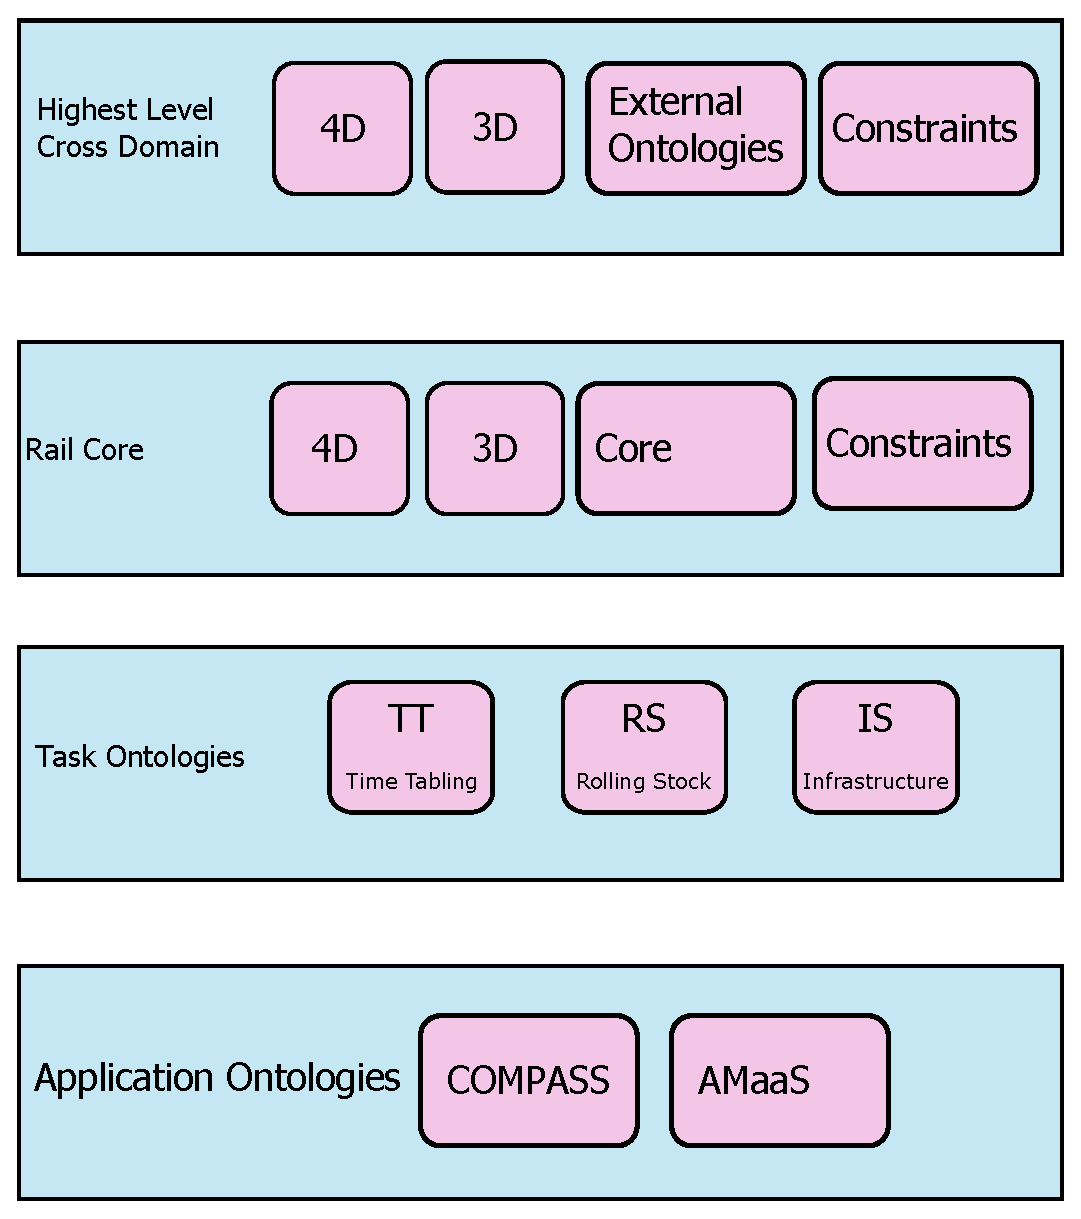
\includegraphics[width=0.6\linewidth,keepaspectratio]{gfx/RacoonLayers}}  
\caption[Racoon Layers]{Structure of the RaCoOn Ontologies. Note the constraints ontologies present on the upper two levels}
\label{fig:RacoonLayers}
\end{figure}

When RaCoOn was designed it was decided that more than one level of expressivity would be required; as stated by \citet{Tutcher2015} ``each semantic module is split into two logical modules: a ‘core’ module containing terminology, T-box relations, and other minimal semantics, and a ‘constraints’ module, containing restrictions on classes and more highly expressive constructs.''. As such the core modules comply with the OWL-RL profile and the constraints, if used, can be implemented in OWL DL, which is more complete and hence more computationally expensive. 

Note that restrictions, which require a higher level of expressivity are placed in separate ontologies which for practical purposes are contained in separate files. These are labelled \say{constraints} in \autoref{fig:RacoonLayers} This allows implementers to use only as much expressivity as their use case requires. This ontology was successfully employed in a project conducted with a commercial partner, and reported in \citet{Tutcher2015a} were data from points machine and wheel impact load detectors was integrated with network layout data and a graphical interface created for it. The industrial partners in this project were then able to extend this to include circuit breaker condition monitoring, with out any further academic input. This was possible because the graphical display element had been designed to display anything that the ontology inferred to be in ``faulty'' condition, all that needed doing was declaring a new type of asset (circuit breaker) and a new fault condition (based on the time to operate). When that condition was met it was displayed in the interface with no code changes being required to the interface. 

\section{Conclusions}

This literature review has found that work is being done to remedy the poor state of data integration within the rail domain in the UK. Data integration has been achieved in the past without use of ontology, however, significantly greater progress is possible. Much work has been done on the development of data models for the European rail domain by a range of projects, the remaining issues are now centred around the take up and use of ontology in the rail domain. Past work has shown there to be value, to many stake holders, from improved systems integration and further more it has been shown that ontology is a good means of achieving that systems integration.  Technology, tools and data models to represent the domain now exist to make implementation of ontology for data integration possible in the rail domain, as shown by the success with which it has been implemented in other domains, most notably biomedical science. 